\documentclass{article}
\usepackage{amsmath}
\usepackage{graphicx}

\begin{document}

\section{Lunar Regolith Properties}

%%%%%%%%%%%%%%%%%%%%%%%%%%%%%%%%%%%%%%%%%%%%%%%%%%%%%%%%%%%%%%%%%%%%%%
\subsection{Porosity}

The lunar regolith porosity is related to the amount of free space between individual grains. The greater the porosity, the more void space is present. Table 3.4.2.3.4-1 of the DSNE gives values of the porosity as a function of depth down to $60$ cm derived from Apollo core measurements (copied from Table 9.5 of the Lunar Sourcebook, \cite{heiken1991lunar}) and shown here in Table \ref{tab:porosity}.


\begin{table}[!htb]
	\begin{center}
		\caption{Porosity for various depths.}
		\label{tab:porosity}
		\begin{tabular}{c c}
			\hline
			Depth Range (cm)  & Average Porosity, n (\%)  \\
			\hline
			$0$ -- $15$  & $52\pm 2$  \\
			$0$ -- $30$  & $49\pm 2$   \\
			$30$ -- $60$ & $44\pm 2$   \\
			$0$ -- $60$  & $46\pm 2$  \\\hline
		\end{tabular}
	\end{center}
\end{table}


%%%%%%%%%%%%%%%%%%%%%%%%%%%%%%%%%%%%%%%%%%%%%%%%%%%%%%%%%%%%%%%%%%%%%%
\subsection{Density}

The bulk density ($\rho$) of the lunar regolith is defined as the mass of material in a given volume, which relates the particle density ($\rho_p$) and porosity ($n$) to the bulk density as (see Section 3.4.2.3.1 of the DSNE or Chapter 9 of the Lunar Sourcebook)
\begin{equation}
\rho = \rho_p(1-n).
\end{equation}

The DSNE suggests using $\rho_p = 3.1$ g/cm$^3$ for the average particle density over the entire Moon. Otherwise, the typical highlands particle density is $\rho_p = 2.75\pm 0.1$ g/cm$^3$ whereas the typical mare particle density is $\rho_p = 3.35\pm 0.1$ g/cm$^3$.

The bulk density\footnote{Follows the average particle density of $3.1$ g/cm$^3$ for all depths with a porosity depth dependence following Table \ref{tab:porosity}, see the \textit{porosity of lunar soil} paragraph on page 492 in the Lunar Sourcebook.} as a function of depth, fit to Apollo data, is given by
\begin{equation}\label{eq:regolith density vs depth}
\rho(z) = 1.92\frac{z+12.2}{z+18},
\end{equation}
where $z$ is the depth in cm and $\rho$ is in units of g/cm$^3$. At the surface ($z=0$), the density is $1.30$ g/cm$^3$, and increases to $1.92$ g/cm$^3$ for large depths. This expression is fairly reasonable down to $3$ m (the limit reached by Apollo drill core samples). In order to get an up-to-depth average of the bulk density, take
\begin{equation}
\rho_{avg, depth}(z) = \frac{1}{z}\int_{0}^{z}dz'\rho(z'), 
\end{equation}
which gives (compare with the equation for $d_m$ on page 494 of the Lunar Sourcebook)
\begin{equation}\label{eq:density depth averaged}
\rho_{avg, depth}(z) = 1.92\left[1 - \frac{5.8\ln\left(\frac{z + 18}{18}\right)}{z}\right].
\end{equation}
For example, the average bulk density of the regolith with a depth range of $0$ -- $60$ cm would be $\rho_{avg, depth}(60)$ = $1.65$ g/cm$^3$.



\begin{figure}[!htb]
	\centering
	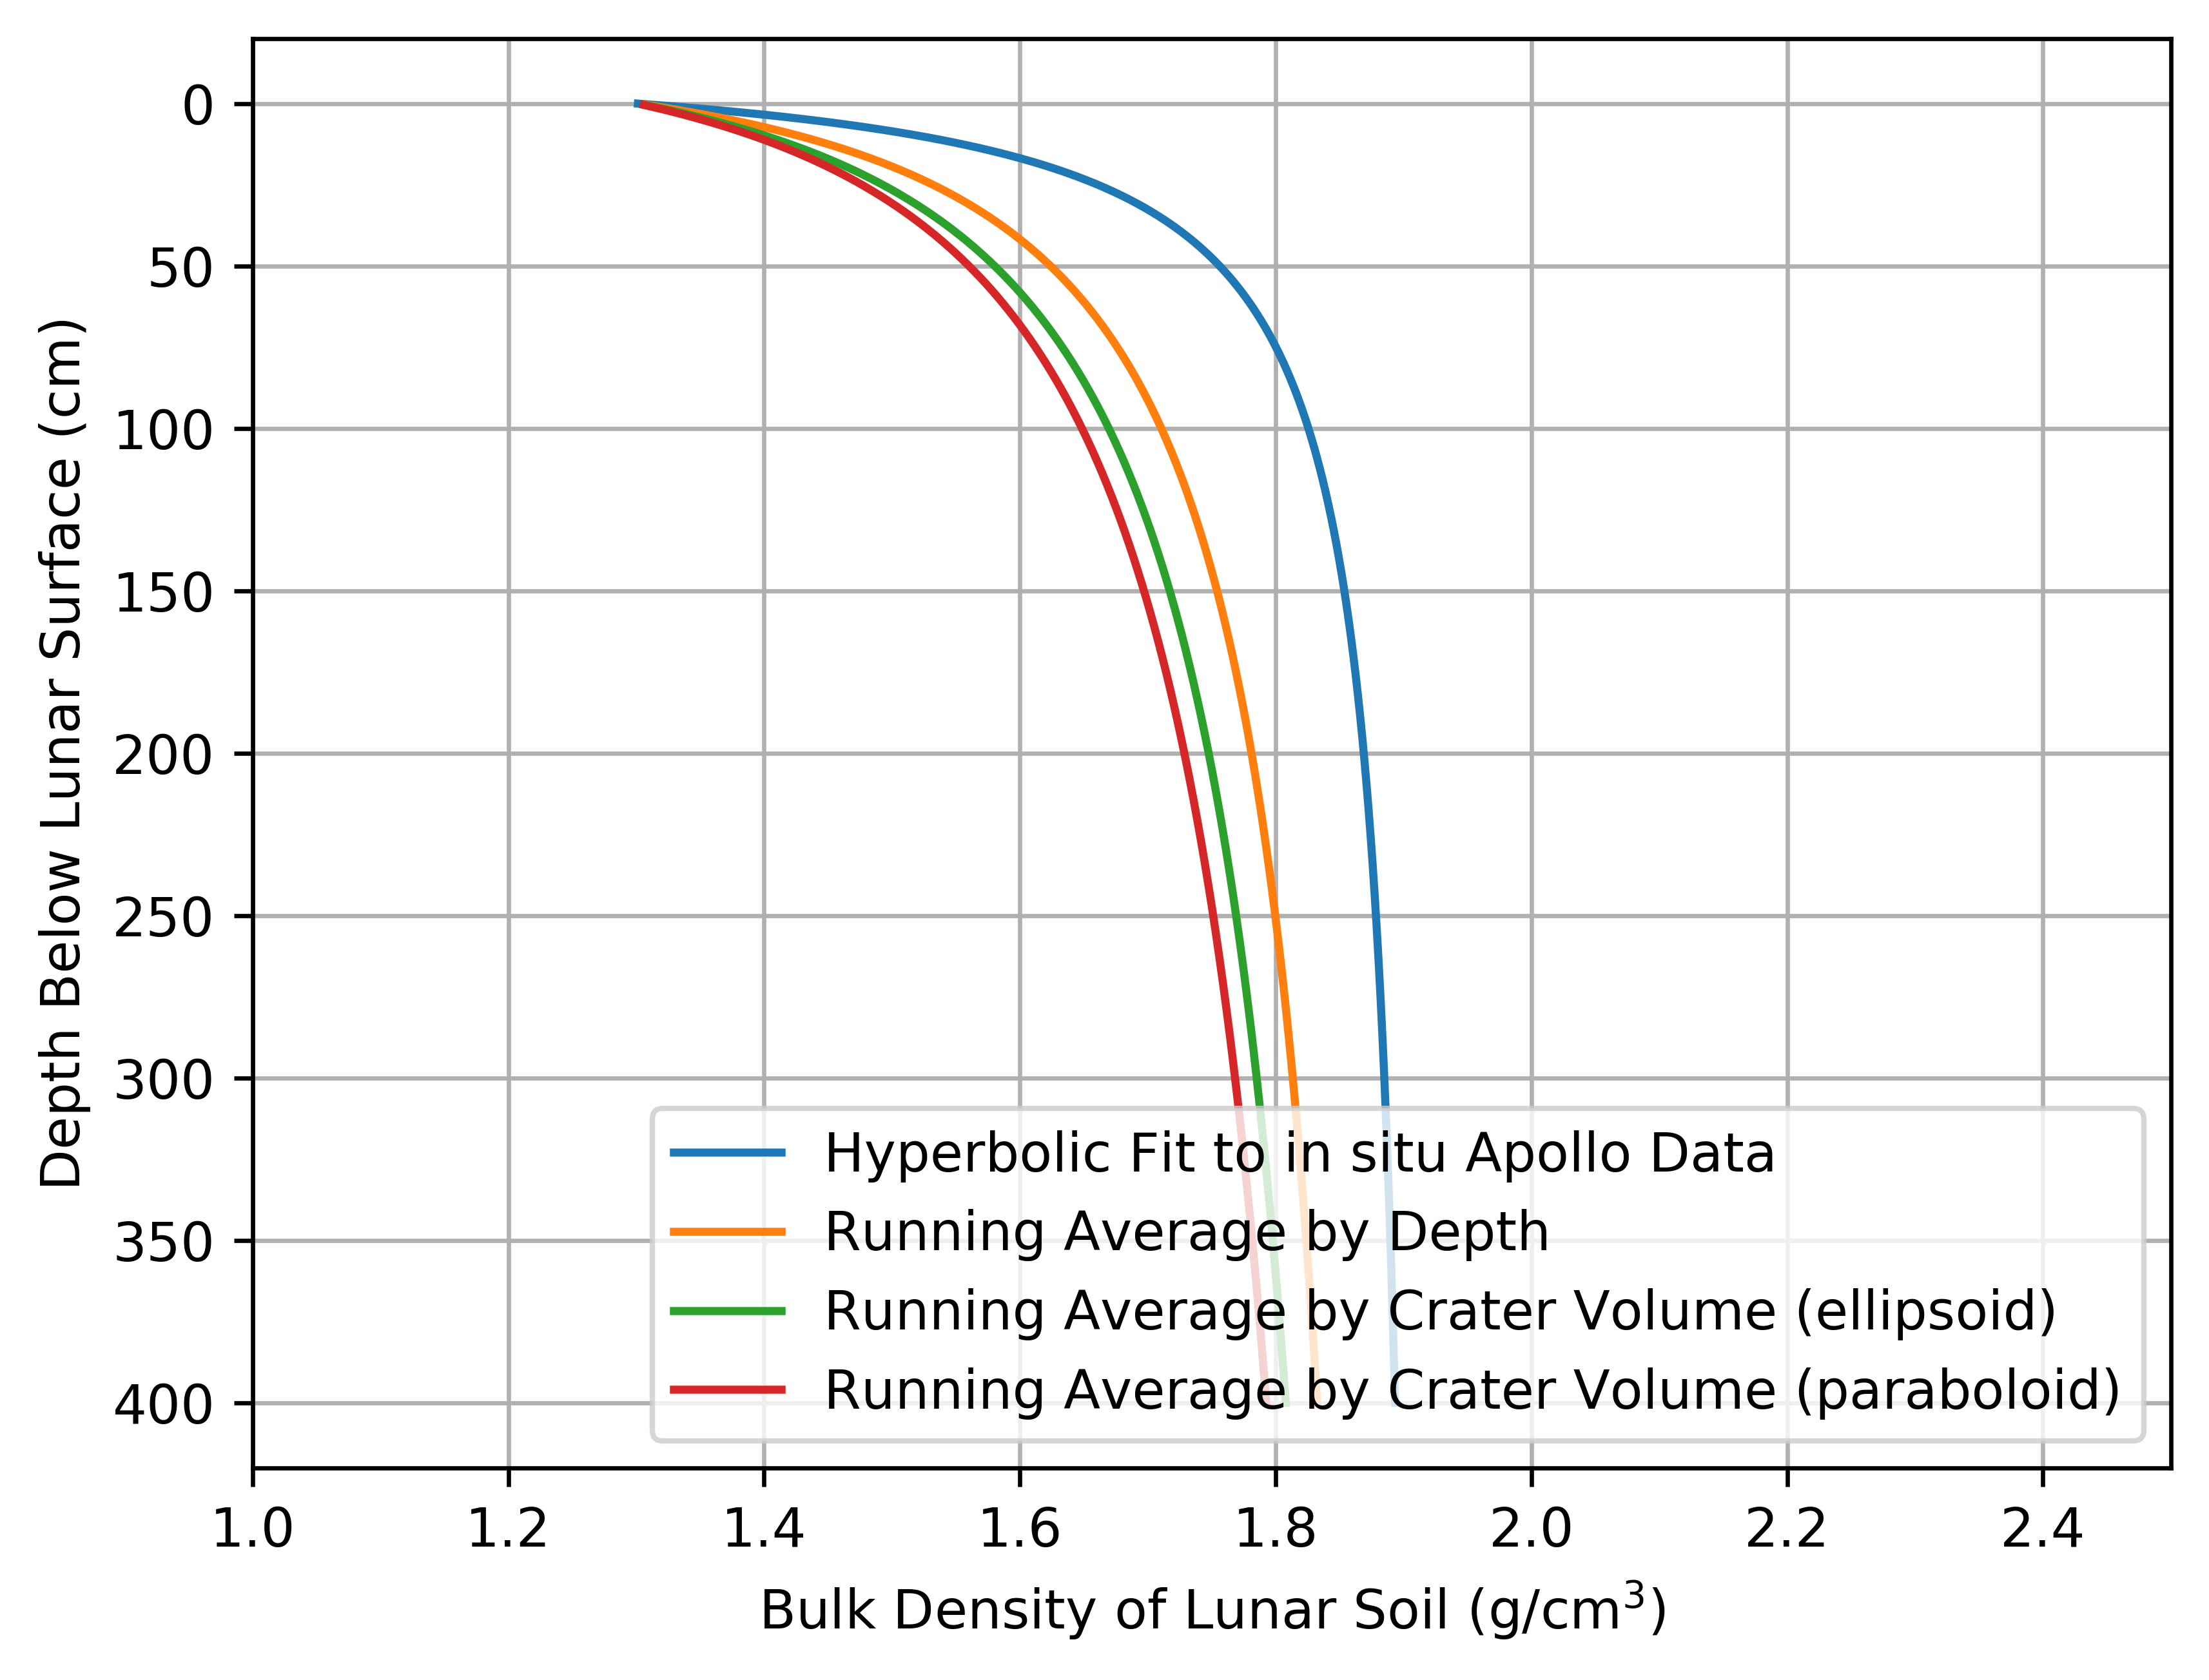
\includegraphics[width=\linewidth]{regolith_density_vs_depth.png}
	\caption{A comparison of the regolith bulk density for a certain depth depth (blue), the depth-averaged bulk density (orange), and the volume-averaged bulk density (green). See also, Figure 9.16 of the Lunar Sourcebook \citep{heiken1991lunar}.}
	\label{fig:regolith_density_vs_depth}
\end{figure}

For a higher-fidelity estimate of the average bulk density sampled by the crater, a volume-average can be used instead of a depth-average, given by
\begin{equation}\label{eq:density volume averaged def}
\rho_{avg, volume}(z) = \frac{\int dV \rho(z')}{\int dV}.
\end{equation}
Expanding the integral in a cylindrical coordinate system and assuming an ellipsoidal crater shape, Equation \eqref{eq:density volume averaged def} becomes
\begin{align}
\rho_{avg, ellipsoid}(z) &= \frac{\int_{0}^{z}\int_{0}^{R\sqrt{1-z'^2/z^2}}\int_{0}^{2\pi}d\phi rdr dz' \rho(z')}{\int_{0}^{z}\int_{0}^{R\sqrt{1-z'^2/z^2}}\int_{0}^{2\pi}d\phi rdr dz'}\\\label{eq:density volume averaged}
&= \frac{1.92}{4z^3}\left[z(6ab - 6b^2 - 3az + 3bz + 4z^2) + 6(a-b)(b^2-z^2)\ln\left(\frac{b}{z + b}\right)\right],
\end{align}
for the volume-averaged density in g/cm$^3$ with $z$ in cm, where $a = 12.2$ and $b = 18$. Following the example from earlier, the average bulk density of the regolith with a depth range of $0$ -- $60$ cm would be $\rho_{avg, ellipsoid}(60)$ = $1.60$ g/cm$^3$, which is $\sim 3\%$ less than $\rho_{avg, depth}(60) = 1.65$ g/cm$^3$.

On the other hand, if a paraboloid crater shape is assumed, Equation \eqref{eq:density volume averaged def} becomes
\begin{align}
\rho_{avg, paraboloid}(z) &= \frac{\int_{0}^{z}\int_{0}^{R\sqrt{1-z'/z}}\int_{0}^{2\pi}d\phi rdr dz' \rho(z')}{\int_{0}^{z}\int_{0}^{R\sqrt{1-z'/z}}\int_{0}^{2\pi}d\phi rdr dz'}\\\label{eq:density volume averaged_para}
&= \frac{1.92}{z/2}\left[b-a + \frac{z}{2} - \frac{(a-b)(b+z)\ln\left(\frac{b}{z+b}\right)}{z}\right],
\end{align}
using the same values for $a$ and $b$ as before. Again, with the prior example, the average bulk density of the regolith with a depth range of $0$ -- $60$ cm would be $\rho_{avg, paraboloid}(60)$ = $1.58$ g/cm$^3$, which is $\sim 4\%$ less than $\rho_{avg, depth}(60) = 1.65$ g/cm$^3$, see Figure \ref{fig:ratio_of_avg_bulk_density}. The expression given in Equation \eqref{eq:density volume averaged_para} is useful for computing the ejected mass from a crater\footnote{In an iterative fashion, since the crater radius depends on the regolith density.}, given a crater depth $z$.





The expressions for the regolith density at a certain depth $z$, weighted by depth, and weighted by crater volume (ellipsoid and paraboloid) are given by Equations \eqref{eq:regolith density vs depth}, \eqref{eq:density depth averaged}, and \eqref{eq:density volume averaged}, \eqref{eq:density volume averaged_para}, respectively, are compared in Figure \ref{fig:regolith_density_vs_depth}. The crater volume is approximated as a half-ellipsoid with two of the dimensions scaled by the crater radius $R$ and one dimension scaled by the crater depth $z$, sliced such that the half-ellipsoid is symmetric about the surface normal for Equation \eqref{eq:density volume averaged}. On the other hand, a paraboloid-shaped crater is used for Equation \eqref{eq:density volume averaged_para}. For a given crater, more of the volume is near the surface so that more weight is given by bulk densities that originate near the surface. In contrast, the depth-averaged bulk density takes the bulk density at each depth equally. This results in the volume-averaged bulk density to be slightly less than the depth-averaged bulk density, as shown in Figure \ref{fig:regolith_density_vs_depth}. In addition, comparing an ellipsoidal crater vs.\ a parabolic crater, the parabolic crater (typically used in literature, see \cite{singer2020lunar}) exhibits the softest increase of the average bulk density as a function of depth.


\begin{figure}[!htb]
	\centering
	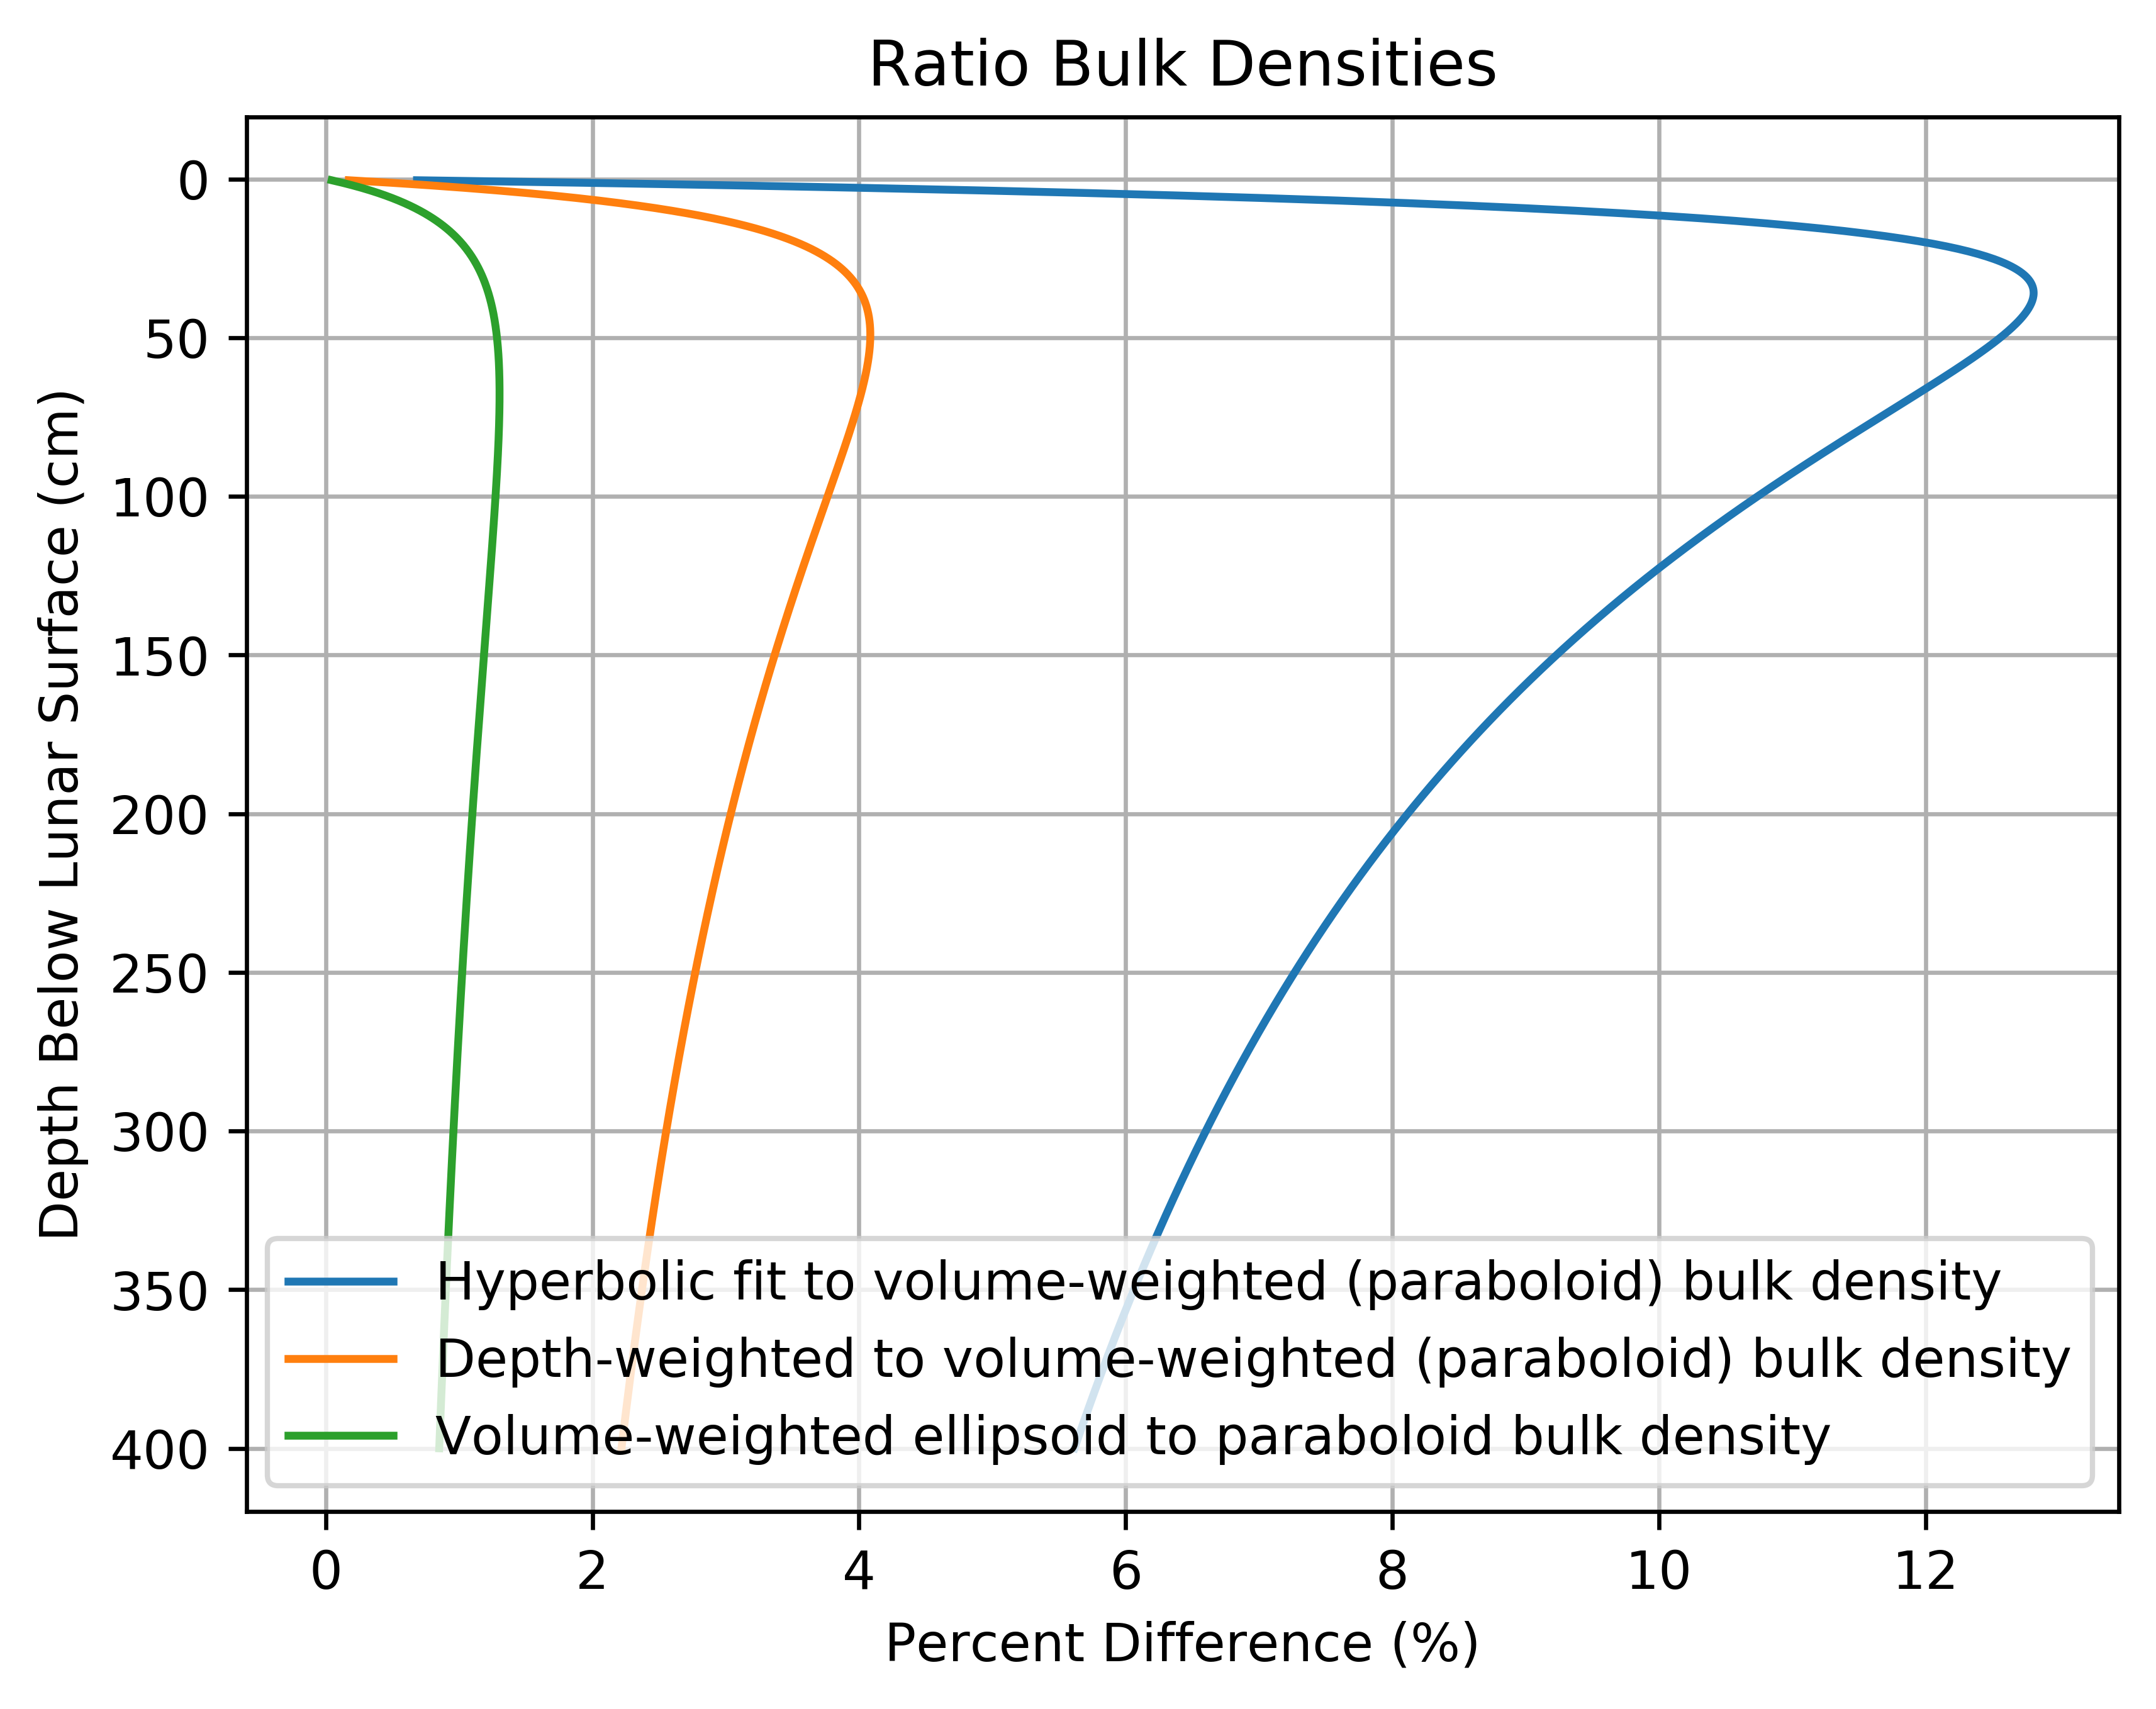
\includegraphics[width=\linewidth]{ratio_of_avg_bulk_density.png}
	\caption{Relative error of using the density at a certain depth (blue) and using the depth-weighted average (orange) of the regolith bulk density.}
	\label{fig:ratio_of_avg_bulk_density}
\end{figure}


%%%%%%%%%%%%%%%%%%%%%%%%%%%%%%%%%%%%%%%%%%%%%%%%%%%%%%%%%%%%%%%%%%%%%%
\subsection{Strength}

The strength of the regolith can be measured in different ways, depending on the use. In the case of modeling impacts, the shear strength of loose regolith and tensile strength of solid rock can be used. The top $10$ m or so consists of fine-grained material called regolith. From $10$ m to about $2$ km is the large scale ejecta that is course grained and ballistically transported (Fig 4.22 of the Lunar Sourcebook, \cite{heiken1991lunar}). All of the impacts studied in this model will create craters less than $2$ km, so it is expected that the shear strength will be used for the loose regolith and large scale ejecta material.

The shear strength of the lunar soil increases with the depth. As an example, both Figure 9.26 of the Lunar Sourcebook, reproduced in Figure \ref{fig:shear_strength_vs_depth}, and Table 12 of \cite{slyuta2014physical} depict this characteristic, shown in Table \ref{tab:shear_strength}.

\begin{table}[!htb]
	\begin{center}
		\caption{The change of the shear strength of the lunar soil with depth.}
		\label{tab:shear_strength}
		\begin{tabular}{c c}
			\hline
			Depth (cm)  & Shear strength (kPa)  \\
			\hline
			$5$  & $0.1$ -- $2.5$  \\
			$50$  & $1$ -- $3.5$   \\
			$100$ & $2$ -- $4$  \\
			$200$  & $4$ -- $8$  \\\hline
		\end{tabular}
	\end{center}
\end{table}

\begin{figure}[!htb]
	\centering
	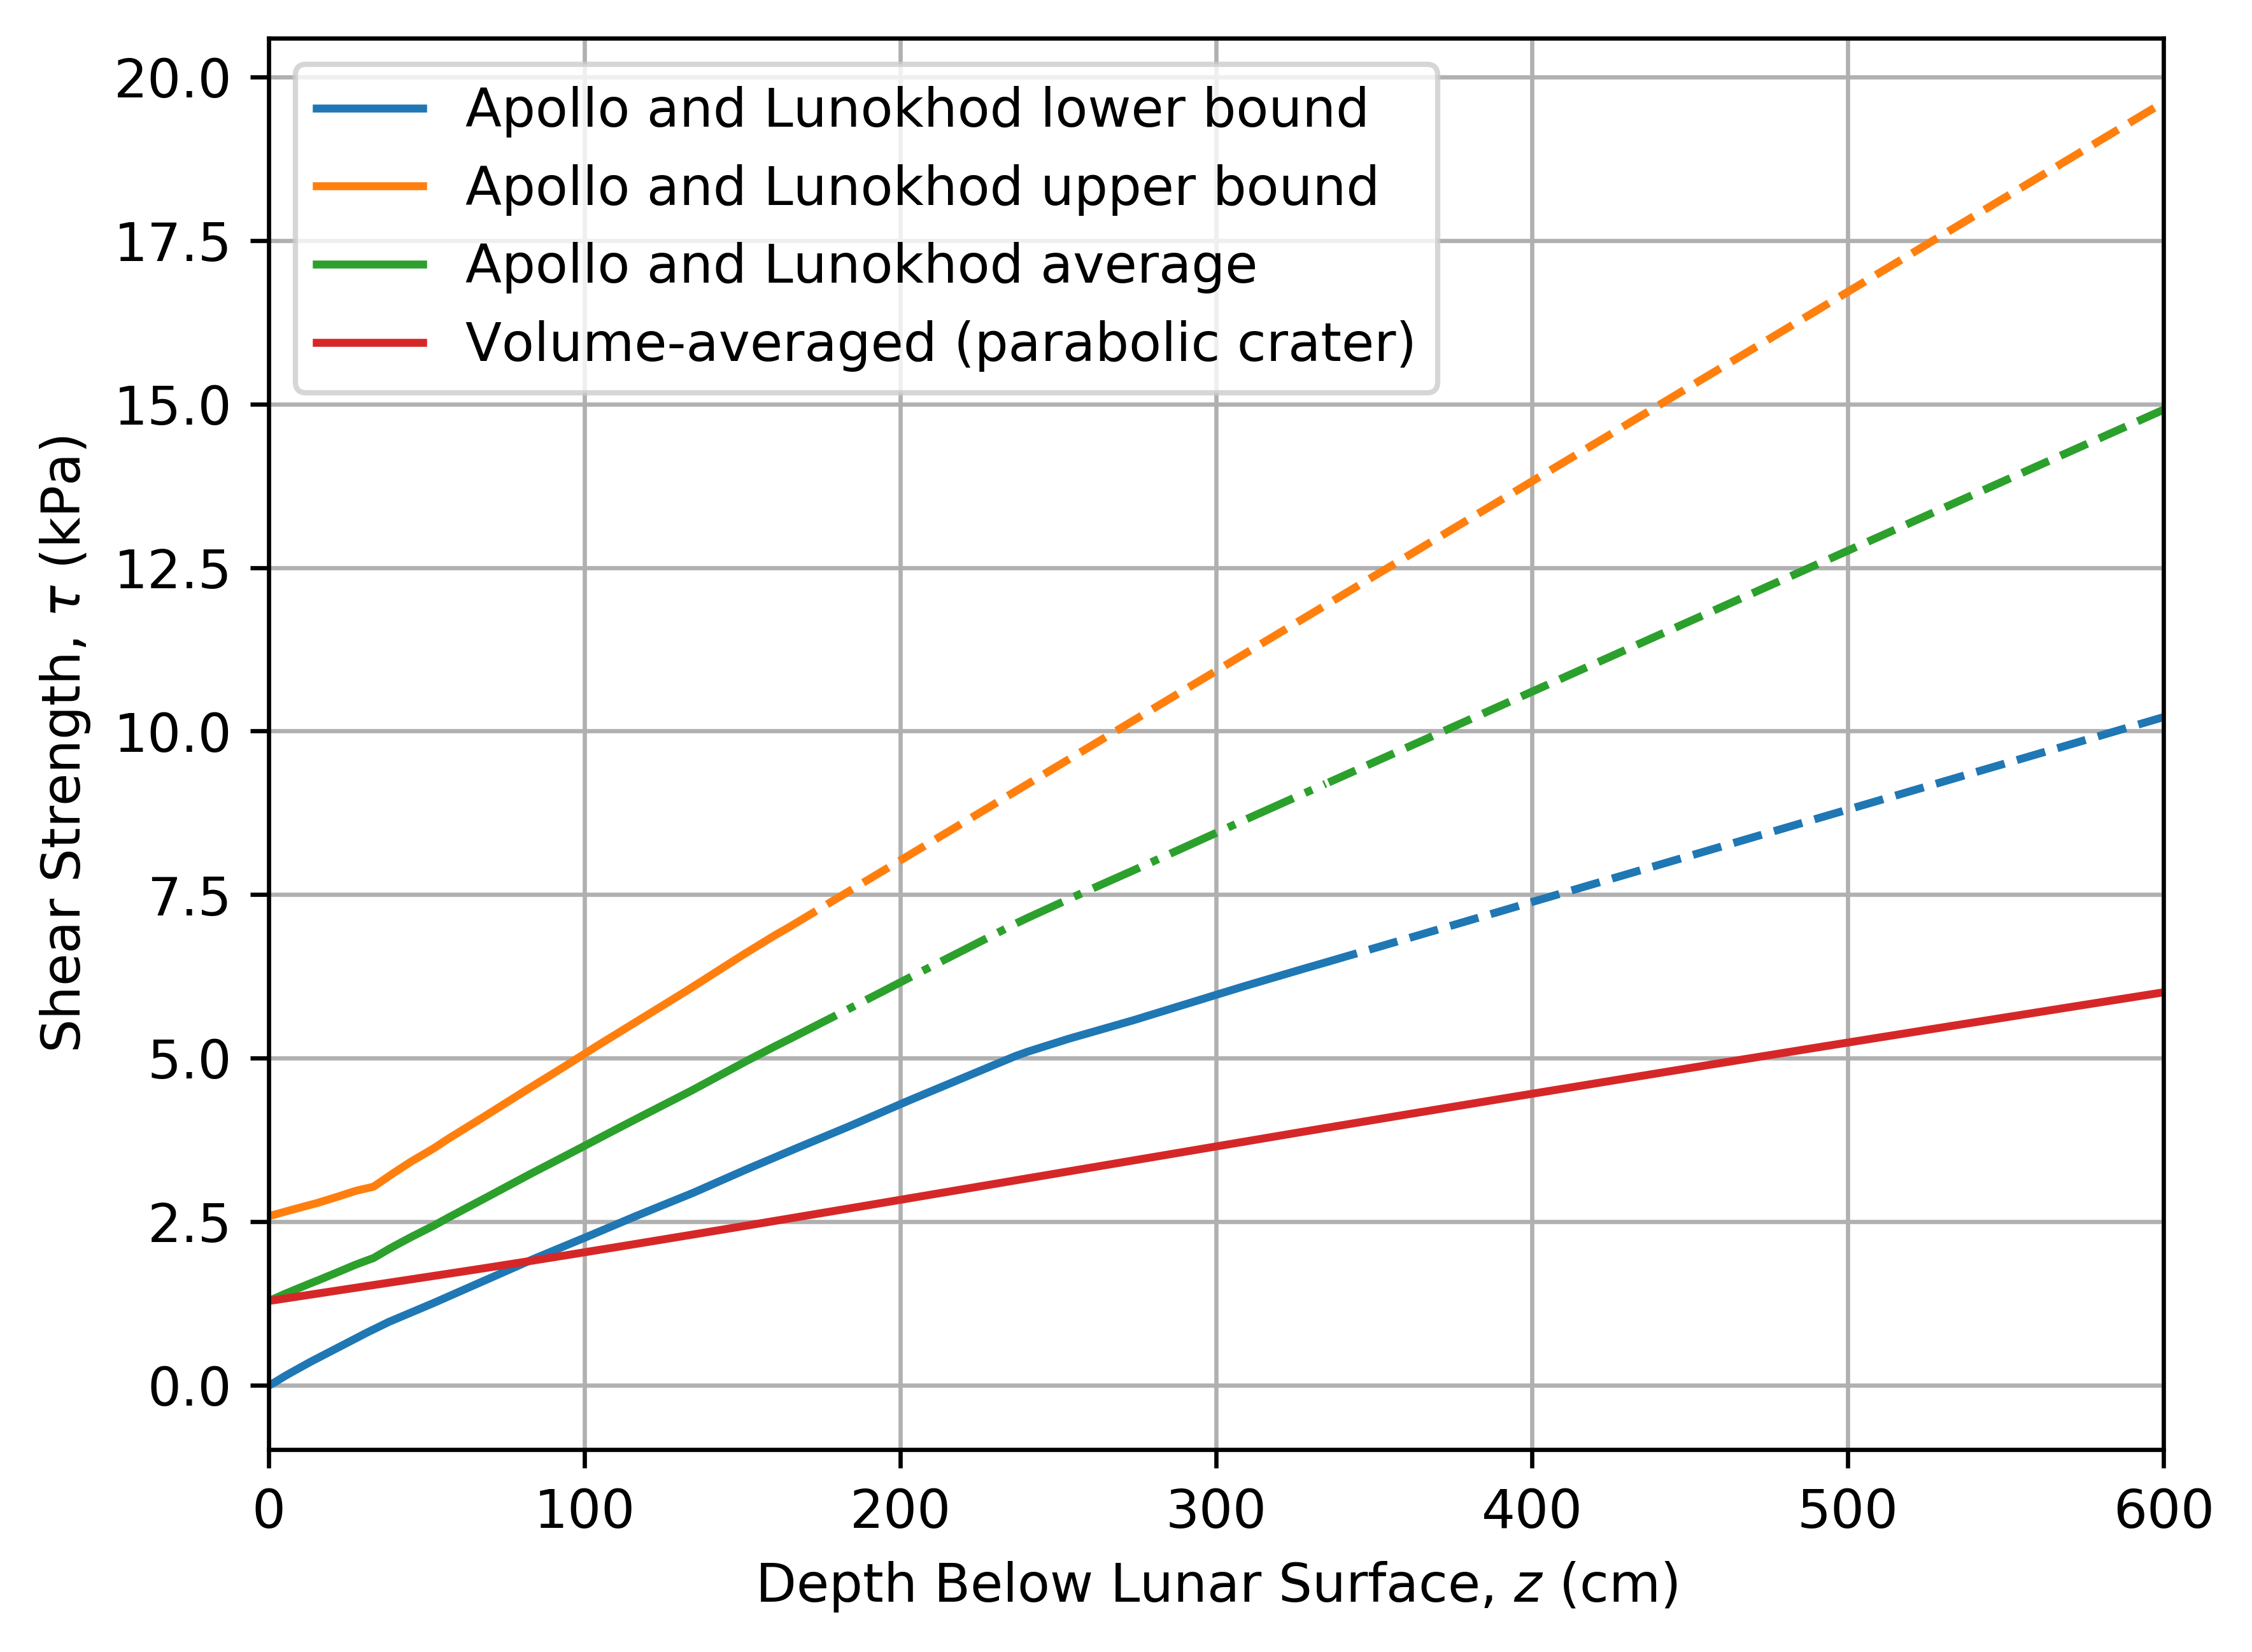
\includegraphics[width=\linewidth]{shear_strength_vs_depth.png}
	\caption{The range of regolith shear strength as a function of depth below the lunar surface taken from Figure 9.26 of the Lunar Sourcebook. The average shear strength is also calculated (green). Points that are extrapolated beyond what is available are shown by the dashed lines. The volume-averaged shear strength (red) assumes a parabolic-shaped crater of depth $z$.}
	\label{fig:shear_strength_vs_depth}
\end{figure}

The average shear strength (green curve) in Figure \ref{fig:shear_strength_vs_depth} can be expressed by the piece-wise form
\begin{equation}\label{eq:shear strength}
\tau(z) =
\begin{cases}
\frac{z}{45.55} + 1.288,\text{   $0 \le z < 50$ cm}\\
\frac{z}{40.21} + 1.144,\text{   $50$ cm $\le z < 250$ cm}\\
\frac{z}{46.06} + 1.942,\text{   $z > 250$ cm}
\end{cases}.
\end{equation}
Assuming the crater has a parabolic shape and that the effective shear strength is the volume-average, Equation \eqref{eq:shear strength} becomes (as shown by the red curve in Figure \ref{fig:shear_strength_vs_depth})
\begin{equation}\label{eq:shear strength_avg_para}
\tau(z) =
\begin{cases}
\frac{z}{136.65} + 1.288,\text{   $0 \le z < 50$ cm}\\
\frac{z}{120.63} + 1.144 + \frac{7.163}{z} - \frac{118.33}{z^2},\text{   $50$ cm $\le z < 250$ cm}\\
\frac{z}{138.18} + 1.942 - \frac{194.81}{z} + \frac{16902}{z^2},\text{   $z > 250$ cm}
\end{cases}.
\end{equation}



%%%%%%%%%%%%%%%%%%%%%%%%%%%%%%%%%%%%%%%%%%%%%%%%%%%%%%%%%%%%%%%%%%%%%%
\subsection{Particle Size Distribution}


%%%%%%%%%%%%%%%%%%%%%%%%%%%%%%%%%%%%%%%%%%%%%%%%%%%%%%%%%%%%%%%%%%%%%%
\subsection{Scaling Law Properties}



\end{document}